\documentclass[12pt]{article}
\usepackage{inputenc}
\usepackage[spanish]{babel}
\decimalpoint % Usar puntos (.) en lugar de comas (,) como separadores decimales
\usepackage{geometry}
\usepackage{amsmath} % Para entornos matemáticos avanzados
\usepackage{amssymb} % Para el uso de \mathbb
\usepackage{amsthm} % Para entornos de teoremas
\usepackage{hyperref} % Para hipervínculos
\usepackage{tikz} % Para diagramas y gráficos
\usepackage{titling}

\newgeometry{left=0.5in, right=0.5in, top=0.25in, bottom=0.25in}

% Definición de entornos personalizados
\newtheorem{problem}{Problema}

\title{Procesos Estocásticos I | Examen Parcial 2}
\author{Semestre 2026-2}
\date{}%25 de abril de 2026}

\begin{document}

\maketitle
\vspace{-1cm}
\small
\textbf{Instrucciones:} Resuelva los siguientes problemas. Encierre sus respuestas finales en un recuadro. 
\begin{problem}
Considere una cadena de Markov con el siguiente diagrama de transición:
\begin{center}
    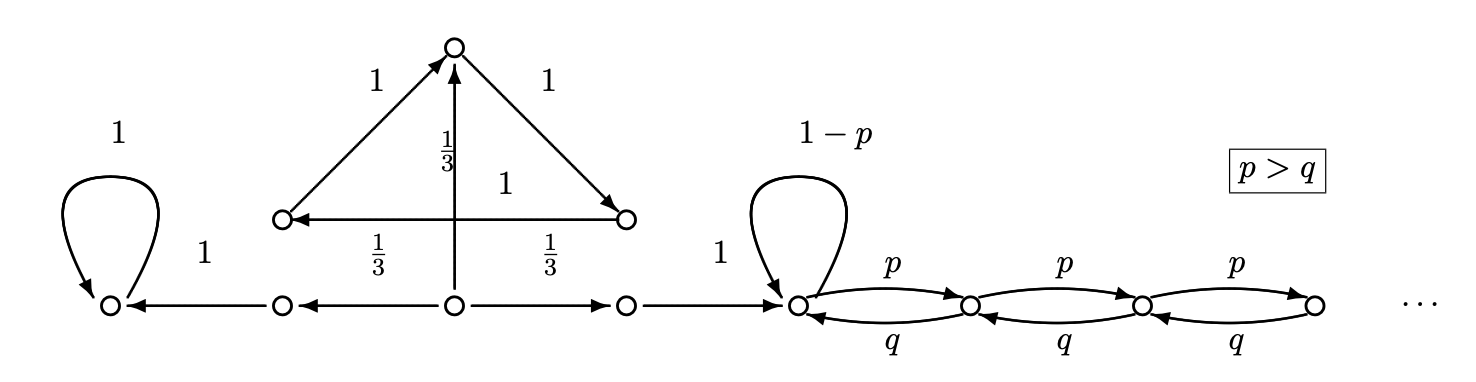
\includegraphics[scale=0.5]{cadena_1.png}
\end{center}    
Identifique todas las clases de comunicación, clasifíquelas como recurrentes positivas, recurrentes nulas o transitorias y calcule su periodo.
\end{problem}

\begin{problem} Para cada enunciado, indique si es verdadero o falso.

\noindent\textbf{(1)} \emph{(Recurrencia como propiedad de clase.)} Sea $\{X_n\}$ una cadena de Markov irreducible. Si para algún estado $i_0 \in S$ se tiene $\mathbb{E}[N_{i_0} \mid X_0 = i_0] = \infty$, entonces todos los estados de la cadena son recurrentes.



\noindent\textbf{(2)} \emph{(Período y distribución estacionaria.)} Toda cadena de Markov irreducible con espacio de estados finito tiene una única distribución estacionaria $\pi$, independientemente de si la cadena es aperiódica o periódica.



\noindent\textbf{(3)} \emph{(Clases cerradas en espacios finitos.)} Existe una cadena de Markov con espacio de estados finito en la que todos los estados son transitorios.



\noindent\textbf{(4)} \emph{(Convergencia y periodicidad.)} Si $\{X_n\}$ es una cadena de Markov irreducible con período $d = 2$, entonces el límite $\lim_{n \to \infty} p_{ij}^{(n)}$ existe para todos los estados $i, j \in S$.



\noindent\textbf{(5)} \emph{(Distribución estacionaria y tiempo medio de retorno.)} Si $\pi$ es la distribución estacionaria de una cadena irreducible y recurrente positiva, entonces $\pi_j > 0$ para todo $j \in S$.



\end{problem}

\begin{problem}
Una clínica veterinaria clasifica a cada paciente en una de tres categorías según su estado de salud al finalizar cada consulta: \textbf{Sano}~(S), \textbf{En tratamiento}~(T) o \textbf{En observación}~(O). De acuerdo con los registros históricos de la clínica, las probabilidades de transición entre visitas son:

\[
P = \begin{pmatrix}
    2/3 & 1/3 & 0   \\[4pt]
    1/4 & 1/2 & 1/4 \\[4pt]
    1/2 & 0   & 1/2
\end{pmatrix},
\]
donde los estados están ordenados como S, T, O.

\begin{enumerate}
    \item[(a)] Un paciente llega hoy clasificado como \textbf{en observación}. ¿Cuál es la probabilidad de que en su segunda consulta a partir de hoy sea clasificado como \textbf{sano}?

    \item[(b)] A largo plazo, ¿qué fracción de las consultas de esta clínica corresponden a pacientes sanos, en tratamiento y en observación, respectivamente?

    \item[(c)] ¿Cuántas consultas pasan en promedio antes de que un paciente que hoy está \textbf{en tratamiento} vuelva a ser clasificado como \textbf{en tratamiento}? ¿Y cuántas para un paciente que hoy está \textbf{en observación}?
\end{enumerate}
\end{problem}

\begin{problem}
Calcule $\displaystyle\lim_{n\to\infty} P^n$, donde
\[
P = \begin{pmatrix}
1/2 & 1/2 & 0   & 0 \\[4pt]
0   & 1/3 & 2/3 & 0 \\[4pt]
1/2 & 0   & 1/2 & 0 \\[4pt]
1/4 & 0   & 3/4 & 0
\end{pmatrix}.
\]
\end{problem}


\newpage

\maketitle
\vspace{-1cm}
\small
\textbf{Instrucciones:} Resuelva los siguientes problemas. Encierre sus respuestas finales en un recuadro. 
\begin{problem}
Considere una cadena de Markov con el siguiente diagrama de transición:
\begin{center}
    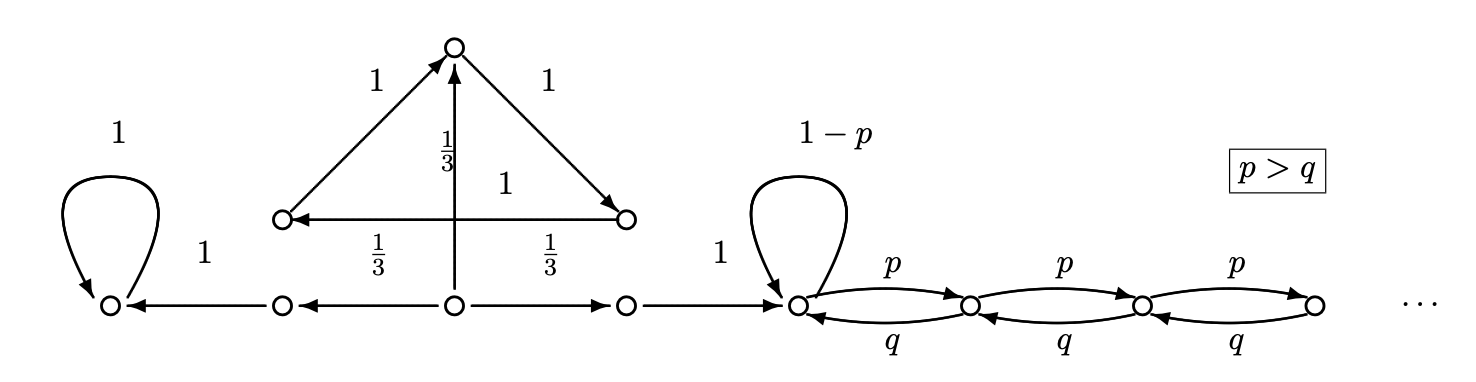
\includegraphics[scale=0.5]{cadena_1.png}
\end{center}    
Identifique todas las clases de comunicación, clasifíquelas como recurrentes positivas, recurrentes nulas o transitorias y calcule su periodo.
\end{problem}

\begin{problem} Para cada enunciado, indique si es verdadero o falso.

\noindent\textbf{(1)} \emph{(Período y distribución estacionaria.)} Toda cadena de Markov irreducible con espacio de estados finito tiene una única distribución estacionaria $\pi$, independientemente de si la cadena es aperiódica o periódica.

\noindent\textbf{(2)} \emph{(Recurrencia como propiedad de clase.)} Sea $\{X_n\}$ una cadena de Markov irreducible. Si para algún estado $i_0 \in S$ se tiene $\mathbb{E}[N_{i_0} \mid X_0 = i_0] = \infty$, entonces todos los estados de la cadena son recurrentes.

\noindent\textbf{(3)} \emph{(Convergencia y periodicidad.)} Si $\{X_n\}$ es una cadena de Markov irreducible con período $d = 2$, entonces el límite $\lim_{n \to \infty} p_{ij}^{(n)}$ existe para todos los estados $i, j \in S$.

\noindent\textbf{(4)} \emph{(Distribución estacionaria y tiempo medio de retorno.)} Si $\pi$ es la distribución estacionaria de una cadena irreducible y recurrente positiva, entonces $\pi_j > 0$ para todo $j \in S$.

\noindent\textbf{(5)} \emph{(Clases cerradas en espacios finitos.)} Existe una cadena de Markov con espacio de estados finito en la que todos los estados son transitorios.



\end{problem}

\begin{problem}
Una clínica veterinaria clasifica a cada paciente en una de tres categorías según su estado de salud al finalizar cada consulta: \textbf{Sano}~(S), \textbf{En tratamiento}~(T) o \textbf{En observación}~(O). De acuerdo con los registros históricos de la clínica, las probabilidades de transición entre visitas son:

\[
P = \begin{pmatrix}
    2/3 & 1/3 & 0   \\[4pt]
    1/4 & 1/2 & 1/4 \\[4pt]
    1/2 & 0   & 1/2
\end{pmatrix},
\]
donde los estados están ordenados como S, T, O.

\begin{enumerate}
    \item[(a)] Un paciente llega hoy clasificado como \textbf{en observación}. ¿Cuál es la probabilidad de que en su segunda consulta a partir de hoy sea clasificado como \textbf{sano}?

    \item[(b)] A largo plazo, ¿qué fracción de las consultas de esta clínica corresponden a pacientes sanos, en tratamiento y en observación, respectivamente?

    \item[(c)] ¿Cuántas consultas pasan en promedio antes de que un paciente que hoy está \textbf{en tratamiento} vuelva a ser clasificado como \textbf{en tratamiento}? ¿Y cuántas para un paciente que hoy está \textbf{en observación}?
\end{enumerate}
\end{problem}

\begin{problem}
Calcule $\displaystyle\lim_{n\to\infty} P^n$, donde
\[
P = \begin{pmatrix}
1/2 & 1/2 & 0   & 0 \\[4pt]
0   & 1/3 & 2/3 & 0 \\[4pt]
1/2 & 0   & 1/2 & 0 \\[4pt]
1/4 & 0   & 3/4 & 0
\end{pmatrix}.
\]
\end{problem}


\end{document}
